\documentclass[10pt,a4paper]{article}
\usepackage[margin=16mm]{geometry}
\usepackage[T1]{fontenc}
\usepackage{lmodern,microtype,graphicx,booktabs,titlesec}
\titleformat{\section}{\large\bfseries}{}{0pt}{}
\titlespacing*{\section}{0pt}{6pt}{3pt}
\usepackage[hidelinks,pdfauthor={},pdftitle={Garbage Collector Benchmarking - Technical Brief Report}]{hyperref}
\setlength{\parindent}{0pt}\setlength{\parskip}{3pt}
\begin{document}
{\LARGE\bfseries Garbage collector benchmarking}\par
{\large Technical Brief Report}\par
This HY446 project compares HotSpot Parallel GC, G1, and ZGC with DaCapo Chopin. The work combines a configuration-driven harness, log processing, aggregation, and tradeoff visualization.
\section*{Experiment and evidence}
The 28 configurations vary 4/8\,GiB heaps, worker counts, and G1 pause targets. The archive holds 616 primary records across 22 workloads; passing markers confirm 560 runs across 20 shared workloads. Cassandra and h2o remain unconfirmed. Headers identify DaCapo 23.11-MR2, OpenJDK 21.0.7, and single-generation ZGC.

The original documents identify Ubuntu 20.04, 16\,GB RAM, an i7-3820 at 3.60\,GHz with eight logical processors, and ten iterations per invocation [R1, p.\,3; R2, p.\,5]. They describe three repetitions, but three complete independent sets are not recoverable. The archive preserves 1,796 text files, separating earlier sidecars from primary logs.
\section*{Additional reported resource results}
The documents provide CPU and memory means for all 28 configurations [R1, pp.\,5, 7, 9; R2, pp.\,8, 11, 14]. Ranges below span configuration means, not confidence intervals.
\begin{center}\small
\begin{tabular}{lrr}\toprule
Collector & Reported mean CPU (s) & Reported mean memory (MB)\\\midrule
Parallel GC & 285.335--289.145 & 1,494.330--2,510.455\\
G1 & 302.025--307.910 & 2,420.975--3,894.240\\
ZGC & 319.920--339.755 & 6,049.905--8,749.430\\\bottomrule
\end{tabular}\end{center}
These are transcribed historical summaries. Per-run resource samples and the collection method are unavailable; memory units remain as printed. They are excluded from the regenerated Pareto analysis.
\section*{Current runtime and pause analysis}
Completed pause-event records support nearest-rank p99 and whole-log pause totals. Concurrent-cycle statistics and event-start lines are excluded; explicit harness-triggered collections remain. Runtime instead comes from the final matching DaCapo passing marker, so runtime and pause axes cover different windows.
\begin{center}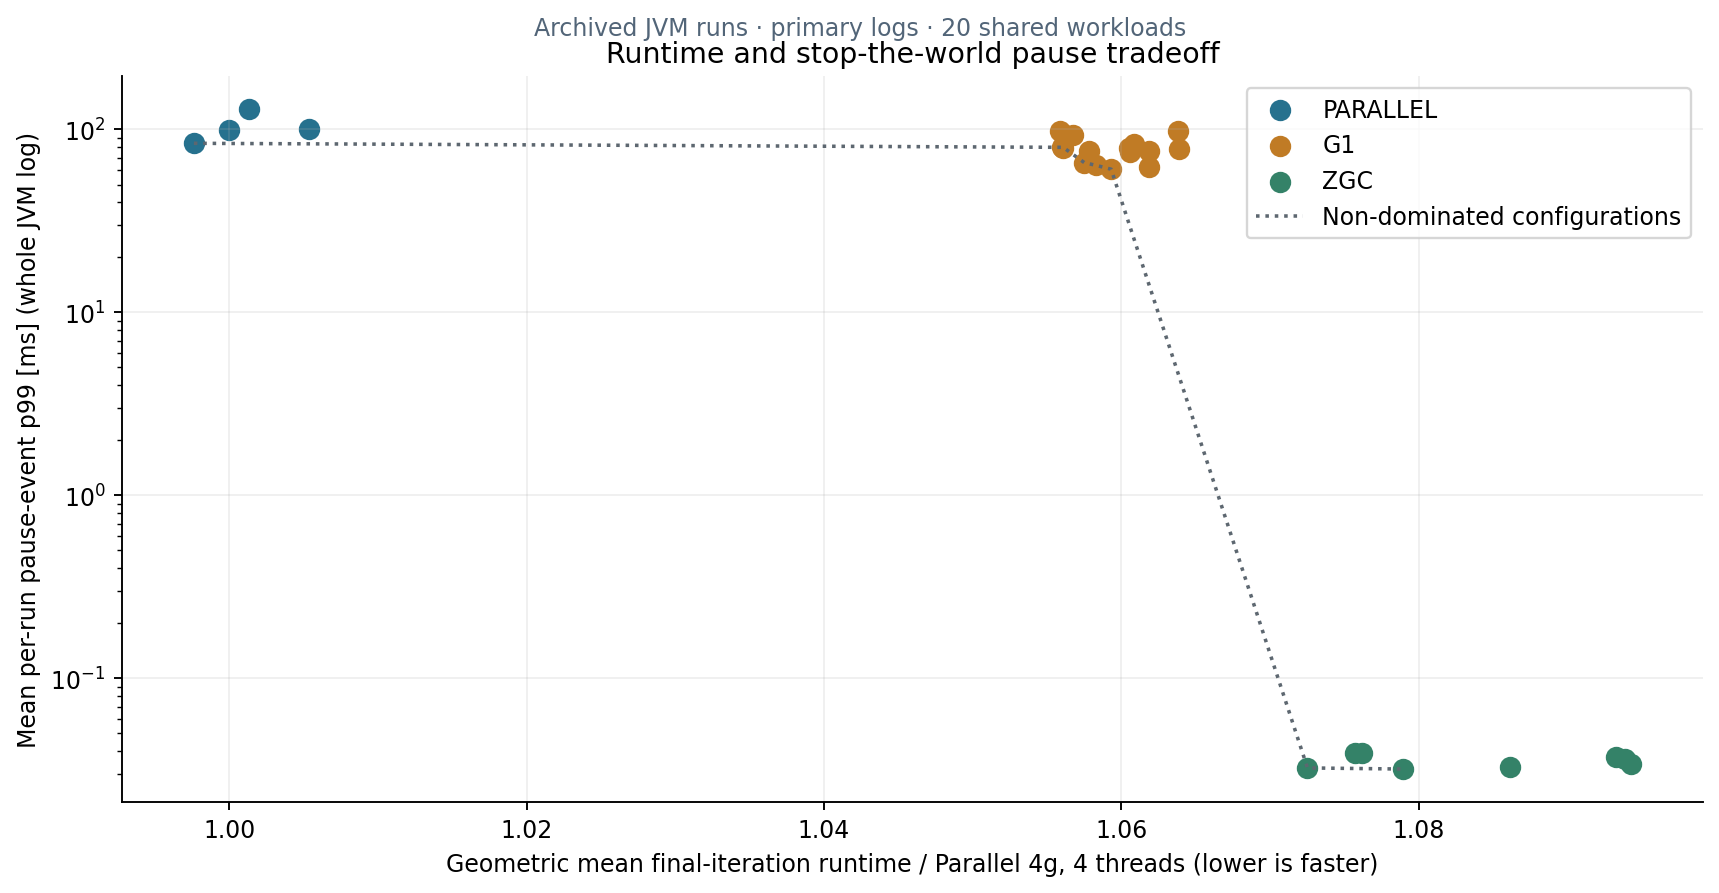
\includegraphics[width=.58\linewidth]{assets/runtime-pauses.png}\end{center}
{\small Runtime is the geometric mean of per-workload ratios to \texttt{parallel-4g-t4}. The pause axis is the mean of per-run p99 values, not a pooled p99 or application-response latency.}

Historical GC percentages mix those windows, and the original ZGC parser reads concurrent-cycle summaries. The documents' derived ``lower-bound overhead'' therefore does not establish a measured zero-GC bound. Current figures use the explicitly scoped reanalysis.
\section*{Verification and references}
Six analysis tests pass. A separate bounded allocation fixture completed with all three collectors on JDK 17; full DaCapo execution was not repeated. Stronger conclusions require aligned phases and controlled, independent repetitions.

{\small [R1] \href{https://github.com/mitsosasim/garbage_collectors_research/blob/main/docs/sources/project-report.pdf}{Original project report} (PDF reading copy; editable ODT retained). [R2] \href{https://github.com/mitsosasim/garbage_collectors_research/blob/main/docs/sources/project-presentation.pdf}{Original presentation}, 19 slides. Figures, references, and the resource CSV are in the \href{https://github.com/mitsosasim/garbage_collectors_research/blob/main/docs/RESEARCH.md}{research guide}; reproduction is in the \href{https://github.com/mitsosasim/garbage_collectors_research/blob/main/docs/SETUP.md}{run guide}.}
\end{document}
